\documentclass[11pt, a4paper, twocolumn]{article}

\usepackage{fancyhdr} % Required for custom headers
\usepackage{extramarks} % Required for headers and footers
\usepackage{graphicx} % Required to insert images
\usepackage{courier} % Required for the courier font
\usepackage[utf8]{inputenc}
\usepackage{datetime}
\usepackage{amsmath}
\usepackage{amssymb}
\usepackage{arydshln}
\usepackage{mathtools}
\usepackage{pgfplots}
\usepackage{tikz}
\usetikzlibrary{arrows,positioning,shapes.geometric}
\usetikzlibrary{plotmarks}
\usepackage[hang,small,bf]{caption}
\usepackage{float}
\usepackage{subcaption}
\usepackage{listings}
\usepackage{hyperref}
\usepackage{epstopdf}
\usepackage[left=1.75cm, right=1.75cm, bottom=3cm, top = 3cm]{geometry}
\usepackage{blindtext}
\usepackage{algorithm}				%För pseudokoder
\usepackage{algpseudocode}			%För pseudokoder
%\usepackage{transparent}
\usepackage{enumitem}
%%\usepackage[table]{xcolor}% http://ctan.org/pkg/xcolor

\newlength\figureheight
\newlength\figurewidth
\newlength\spacing

%%%%%%%%%%%%%%%%%%%%%%% FOR DRAFT %%%%%%%%%%%%%%%%%%%%%%%%%%
\newcommand{\printdraft}{0} % If we want to print draft
%%% USAGE IN TEXT:
% 	\ifnum\printdraft>0
% 		OUR DRAFT TEXT GOES HERE
% 	\else
%   \begin{center}
%   	\textbf{--- DRAFT PARTS ---}
%   \end{center}
%   \fi
%%%%%%%%%%%%%%%%%%%%%%% END DRAFT %%%%%%%%%%%%%%%%%%%%%%%%%%
\linespread{1.0} % Line spacing

% Set up the header and footer
%\pagestyle{fancy}
\lhead{J. Sahlström, A. Lindström \& D. Dürebrandt\\ \today} % Top left header
\rhead{Project in Modelling Complex Systems} % Right center head
\chead{\firstxmark} % Center right header
\lfoot{\lastxmark} % Bottom left footer
\cfoot{\thepage} % Bottom center footer
%\rfoot{Page\ \thepage\ \protect\pageref{LastPage}} % Bottom right footer
\renewcommand\headrulewidth{0.4pt} % Size of the header rule
\renewcommand\footrulewidth{0.4pt} % Size of the footer rule
\newcommand\bigforall{\mbox{\LARGE $\mathsurround0pt\forall$}}  % Large for all symbol
\setlength{\columnsep}{30pt}
\setlength\parindent{0pt} % Removes all indentation from paragraphs

%----------------------------------------------------------------------------------------
%   TITLE PAGE
%----------------------------------------------------------------------------------------

\title{
%
\includegraphics[width=0.3\textwidth]{../img/uu-logo.pdf}\\
Decision-making in Traveling Animal Groups \\ \Large \emph{Project in Modelling Complex Systems}}
\author{
Jakob Sahlström \\ \scriptsize{jasa5691@student.uu.se} 
\and
Anders Lindström \\ \scriptsize{anli6945@student.uu.se} 
\and
Jesper Dürebrandt \\ \scriptsize{jedu6357@student.uu.se}
}
\date{Uppsala University\\\ \\\today} % Insert date here if you want it to appear below your name

%----------------------------------------------------------------------------------------

\usepackage{eso-pic}
\newcommand\BackgroundPic{%
\put(0,0){%
\parbox[b][1.66\paperheight]{\paperwidth}{%
\vfill
\centering

\includegraphics[width=.8\paperwidth,height=.8\paperheight,trim=0 40 0 0, clip,%
keepaspectratio]{img/uu-logo3.pdf}%
%{\transparent{0.20}
\includegraphics[width=.8\paperwidth,height=.8\paperheight,trim=0 40 0 0, clip,%
%keepaspectratio]{img/uu-logo.pdf}}%
\vfill
}}}

\begin{document}
\AddToShipoutPicture*{\BackgroundPic}
\twocolumn[
\begin{@twocolumnfalse}
\maketitle
% \begin{abstract}
% \input{sections/abstract.tex}
% \end{abstract}
\end{@twocolumnfalse}
]
%\maketitle
%\thispagestyle{empty}
%\newpage
\setcounter{page}{1}
%\newpage
% \tableofcontents
% \newpage

\section{Model Description}
% A group contains $N$ individuals, where each individual $i$ has a position vector $\boldsymbol{c}_i(t)$, direction as a scalar $d_i(t)$ defined as counter-clockwise angle from the positive x-axis, and speed $s$. 
% The individuals avoid collisions with their neighbors by turning away from individuals $j$ within distance $\alpha$ according to
% \begin{equation}
% d_i (t+\Delta t) = \arg \left(- \sum_{j \neq i} \frac{\boldsymbol{c}_j (t) - \boldsymbol{c}_i (t)}{|\boldsymbol{c}_j (t) - \boldsymbol{c}_i (t) |}\right),
% \label{eq:repulsion}
% \end{equation}
%  where $\arg$ refer to angle to the positive x-axis of of the resulting vector inside the parenthesis and $d_i(t)$ is the desired direction of motion. 
%  If there are no neighbors within distance $\alpha$, the individuals will move towards individuals $j$ within distance $\rho$ according to
% \begin{equation}
% d_p (t) = \arg \left(\sum_{j \neq i} \frac{\boldsymbol{c}_j (t)- \boldsymbol{c}_i (t)}{|\boldsymbol{c}_j (t) - \boldsymbol{c}_i (t)|} \right),
% \label{eq:dp}
% \end{equation}

% \begin{equation}
% d_d (t) = \text{mean}\left( \sum_{j = 1} d_j (t) \right),
% \label{eq:dd}
% \end{equation}

% \begin{equation}
% d_i (t+\Delta t) = \frac{d_p (t) + d_d (t)}{2}.
% \label{eq:attraction}
% \end{equation}
% Here $d_p$ is the direction from individual $i$ to individual $j$, and $d_d$ is the mean value of the directions of the individuals $j$.
% A proportion $p$ of the individuals know in which direction $g$ to go, and their desired direction is given by
% \begin{equation}
% d_i^\prime (t+\Delta t) = d_i (t+\Delta t) + \omega (g - d_i (t+\Delta t)),
% \label{eq:attraction}
% \end{equation}
% where $\omega$ decides the influence of the known direction $g$; $\omega=0$ makes the individual move only by social interaction and the higher the value of $\omega$, the more the individual moves in the known direction.
% \\\\
% A small random angle $\theta$ is added to 

A group contains $N$ individuals, where each individual $i$ has a position vector $\boldsymbol{c}_i(t)$, direction vector $\boldsymbol{v}_i(t)$ and speed $s$. 
The individuals avoid collisions with their neighbors by turning away from individuals $j$ within distance $\alpha$ according to
\begin{equation}
\boldsymbol{d}_i (t+\Delta t) = - \sum_{j \neq i} \frac{\boldsymbol{c}_j (t) - \boldsymbol{c}_i (t)}{|\boldsymbol{c}_j (t) - \boldsymbol{c}_i (t) |},
\label{eq:repulsion}
\end{equation}
where $\boldsymbol{d}_i(t)$ is the desired direction of motion. 
If there are no neighbors within distance $\alpha$, the individuals will move towards individuals $j$ within distance $\rho$ according to
\begin{equation}
\boldsymbol{d}_i (t+\Delta t) = \sum_{j \neq i} \frac{\boldsymbol{c}_j (t)- \boldsymbol{c}_i (t)}{|\boldsymbol{c}_j (t) - \boldsymbol{c}_i (t)|} + \sum_{j = 1} \frac{\boldsymbol{v}_j (t)}{|\boldsymbol{v}_j (t)|}.
\label{eq:attraction}
\end{equation}
The direction $\boldsymbol{d}_i(t)$ is normalized to a unit vector $\hat{\boldsymbol{d}}_i(t)$. 
A proportion $p$ of the individuals know in which direction $\hat{\boldsymbol{g}}$ to go, and their desired direction is given by
\begin{equation}
\boldsymbol{d}_i^\prime (t+\Delta t) = \frac{\hat{\boldsymbol{d}}_i (t+\Delta t) + \omega \hat{\boldsymbol{g}}}{|\hat{\boldsymbol{d}}_i (t+\Delta t) + \omega \hat{\boldsymbol{g}}|},
\label{eq:attraction}
\end{equation}
where $\omega$ decides the influence of the known direction $\hat{\boldsymbol{g}}$; $\omega=0$ makes the individual move only by social interaction and the higher the value of $\omega$, the more the individual moves in the known direction.
\\\\
The direction of each individual is rotated by a small random angle, picked from a normal distribution with mean zero and standard deviation 0.01, in order to simulate stochastic factors that make impact on the movement of the group. 

\subsection{Movement} % (fold)
\label{sub:movement}
In each time step an individual can change its direction by a maximum of $\theta \Delta t$. 
If the difference in angle between its calculated wanted new direction $\boldsymbol{d}_i''$ and its current direction is lower than $\theta \Delta t$, its velocity will be set to $\boldsymbol{v}_i(t + \Delta t) = \boldsymbol{d}_i''$.
If it is higher, it will be changing its direction angle with $\theta \Delta t$ towards direction $\boldsymbol{d}_i''$. 
The new velocity $\boldsymbol{v}_i(t + \Delta t)$ will then be used to calculate the new position, as 
\begin{equation}
	\boldsymbol{c}_i(t+\Delta t) = \boldsymbol{c}_i(t) + \boldsymbol{v}_i(t + \Delta t)\Delta t s_i,
\end{equation}
where $s_i$ is the speed of the individual
% subsection movement (end)

\subsection{Elongation} % (fold)
\label{sub:elongation}
A bounding box is calculated for given time steps, which is defined as the smallest box that can contain all individuals in the simulations, having one side parallel to the mean direction of the group in that time step, and the other side perpendicular.
The elongation is defined as the length of the parallel side divided the length of the perpendicular side.
% subsection elongation (end)

\section{Simulation Results}

\setlength\figurewidth{0.58\linewidth}
\setlength\figureheight{0.58\linewidth}

\begin{figure}[H]
%\centering
\tikzstyle{every node}=[font=\scriptsize]
% This file was created by matlab2tikz v0.4.7 running on MATLAB 8.2.
% Copyright (c) 2008--2014, Nico Schlmer <nico.schloemer@gmail.com>
% All rights reserved.
% Minimal pgfplots version: 1.3
% 
% The latest updates can be retrieved from
%   http://www.mathworks.com/matlabcentral/fileexchange/22022-matlab2tikz
% where you can also make suggestions and rate matlab2tikz.
% 
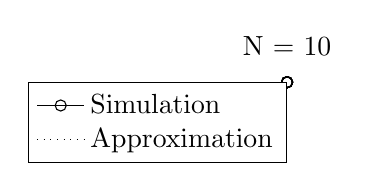
\begin{tikzpicture}

\begin{axis}[%
width=\figurewidth,
height=\figureheight,
unbounded coords=jump,
scale only axis,
xmin=0,
xmax=1,
xlabel={Proportion of informed individuals},
ymin=0,
ymax=10,
ylabel={Elongation},
title={N = 10},
legend style={draw=black,fill=white,legend cell align=left}
]
\addplot [color=black,solid,mark=o,mark options={solid}]
  table[row sep=crcr]{0	0.994143373720641\\
0.1	1.02550613285966\\
0.2	1.20640748601818\\
0.3	1.28533038624398\\
0.4	1.65159642101851\\
0.5	1.8607210442573\\
0.6	1.73468615483567\\
0.7	1.82915697876139\\
0.8	1.74592126576703\\
0.9	1.42801543588063\\
1	1.42268691375327\\
};
\addlegendentry{Simulation};

\addplot [color=black,dotted]
  table[row sep=crcr]{0	-inf\\
0.1	-44.8700576850888\\
0.2	inf\\
0.3	31.8804418757714\\
0.4	14.6568542494924\\
0.5	9.16227766016838\\
0.6	6.52072594216369\\
0.7	4.98975845794461\\
0.8	4\\
0.9	3.31220710410019\\
1	2.80901699437495\\
};
\addlegendentry{Approximation};

\end{axis}
\end{tikzpicture}%
\caption{Actual distribution in box.}
\label{fig:elong10}
\end{figure}

\begin{figure}[H]
%\centering
\tikzstyle{every node}=[font=\scriptsize]
% This file was created by matlab2tikz v0.4.3.
% Copyright (c) 2008--2013, Nico Schlmer <nico.schloemer@gmail.com>
% All rights reserved.
% 
% The latest updates can be retrieved from
%   http://www.mathworks.com/matlabcentral/fileexchange/22022-matlab2tikz
% where you can also make suggestions and rate matlab2tikz.
% 
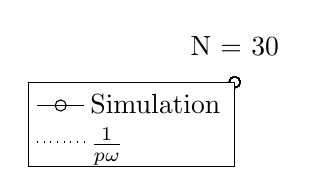
\begin{tikzpicture}

\begin{axis}[%
width=\figurewidth,
height=\figureheight,
unbounded coords=jump,
scale only axis,
xmin=0,
xmax=1,
xlabel={Proportion of informed individuals},
ymin=0,
ymax=10,
ylabel={Elongation},
title={N = 30},
legend style={draw=black,fill=white,legend cell align=left}
]
\addplot [
color=black,
solid,
mark=o,
mark options={solid}
]
table[row sep=crcr]{
0 1.00301535072817\\
0.1 1.03205098421723\\
0.2 1.29504911983557\\
0.3 3.09125904689578\\
0.4 3.00358256435899\\
0.5 2.78090658125569\\
0.6 2.36526002042314\\
0.7 2.04992392129237\\
0.8 1.78922882325996\\
0.9 1.36911901935186\\
1 1.20710100939255\\
};
\addlegendentry{Simulation};

\addplot [
color=black,
dotted
]
table[row sep=crcr]{
0 inf\\
0.1 20\\
0.2 10\\
0.3 6.66666666666667\\
0.4 5\\
0.5 4\\
0.6 3.33333333333333\\
0.7 2.85714285714286\\
0.8 2.5\\
0.9 2.22222222222222\\
1 2\\
};
\addlegendentry{$\frac{1}{p\omega}$};

\end{axis}
\end{tikzpicture}%
\caption{Approximated distribution.}
\label{fig:elong30}
\end{figure}

\begin{figure}[H]
%\centering
\tikzstyle{every node}=[font=\scriptsize]
% This file was created by matlab2tikz v0.4.3.
% Copyright (c) 2008--2013, Nico Schlmer <nico.schloemer@gmail.com>
% All rights reserved.
% 
% The latest updates can be retrieved from
%   http://www.mathworks.com/matlabcentral/fileexchange/22022-matlab2tikz
% where you can also make suggestions and rate matlab2tikz.
% 
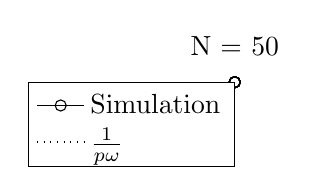
\begin{tikzpicture}

\begin{axis}[%
width=\figurewidth,
height=\figureheight,
unbounded coords=jump,
scale only axis,
xmin=0,
xmax=1,
xlabel={Proportion of informed individuals},
ymin=0,
ymax=10,
ylabel={Elongation},
title={N = 50},
legend style={draw=black,fill=white,legend cell align=left}
]
\addplot [
color=black,
solid,
mark=o,
mark options={solid}
]
table[row sep=crcr]{
0 1.02034692352163\\
0.1 1.09289035466909\\
0.2 1.20577695632396\\
0.3 3.95680389947455\\
0.4 3.72778674107091\\
0.5 3.55498346370831\\
0.6 2.96997739867156\\
0.7 2.47071768260361\\
0.8 1.9452728503174\\
0.9 1.67910478982234\\
1 1.50828773014056\\
};
\addlegendentry{Simulation};

\addplot [
color=black,
dotted
]
table[row sep=crcr]{
0 inf\\
0.1 20\\
0.2 10\\
0.3 6.66666666666667\\
0.4 5\\
0.5 4\\
0.6 3.33333333333333\\
0.7 2.85714285714286\\
0.8 2.5\\
0.9 2.22222222222222\\
1 2\\
};
\addlegendentry{$\frac{1}{p\omega}$};

\end{axis}
\end{tikzpicture}%
\caption{Approximated distribution.}
\label{fig:elong50}
\end{figure}

\begin{figure}[H]
%\centering
\tikzstyle{every node}=[font=\scriptsize]
% This file was created by matlab2tikz v0.4.3.
% Copyright (c) 2008--2013, Nico Schlmer <nico.schloemer@gmail.com>
% All rights reserved.
% 
% The latest updates can be retrieved from
%   http://www.mathworks.com/matlabcentral/fileexchange/22022-matlab2tikz
% where you can also make suggestions and rate matlab2tikz.
% 
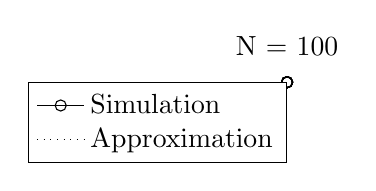
\begin{tikzpicture}

\begin{axis}[%
width=\figurewidth,
height=\figureheight,
unbounded coords=jump,
scale only axis,
xmin=0,
xmax=1,
xlabel={Proportion of informed individuals},
ymin=0,
ymax=10,
ylabel={Elongation},
title={N = 100},
legend style={draw=black,fill=white,legend cell align=left}
]
\addplot [
color=black,
solid,
mark=o,
mark options={solid}
]
table[row sep=crcr]{
0 0.99547989327611\\
0.1 1.08654334799565\\
0.2 6.53913064364081\\
0.3 8.169192332035\\
0.4 5.22493239088512\\
0.5 5.08763539124752\\
0.6 4.30158665907168\\
0.7 3.48136690684954\\
0.8 2.87218165405375\\
0.9 2.27742230081664\\
1 1.79634021711085\\
};
\addlegendentry{Simulation};

\addplot [
color=black,
dotted
]
table[row sep=crcr]{
0 inf\\
0.1 20\\
0.2 10\\
0.3 6.66666666666667\\
0.4 5\\
0.5 4\\
0.6 3.33333333333333\\
0.7 2.85714285714286\\
0.8 2.5\\
0.9 2.22222222222222\\
1 2\\
};
\addlegendentry{Approximation};

\end{axis}
\end{tikzpicture}%
\caption{Approximated distribution.}
\label{fig:elong100}
\end{figure}
\vfill

\setlength\figurewidth{0.65\linewidth}
\setlength\figureheight{0.65\linewidth}

\begin{figure}[H]
%\centering
\tikzstyle{every node}=[font=\scriptsize]
% This file was created by matlab2tikz v0.4.3.
% Copyright (c) 2008--2013, Nico Schlmer <nico.schloemer@gmail.com>
% All rights reserved.
% 
% The latest updates can be retrieved from
%   http://www.mathworks.com/matlabcentral/fileexchange/22022-matlab2tikz
% where you can also make suggestions and rate matlab2tikz.
% 
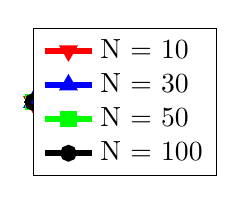
\begin{tikzpicture}

\begin{axis}[%
width=\figurewidth,
height=\figureheight,
scale only axis,
xmin=0,
xmax=1,
xlabel={Proportion of informed individuals, p},
ymin=0,
ymax=1.1,
ylabel={Accuracy},
axis x line*=bottom,
axis y line*=left,
legend style={at={(0.6,0.5)},anchor=west,draw=black,fill=white,legend cell align=left}
]
\addplot [
color=red,
solid,
line width=2.0pt,
mark=triangle,
mark options={solid,,rotate=180}
]
table[row sep=crcr]{
0 0.403156228560285\\
0.1 0.595839630695204\\
0.2 0.884699864455051\\
0.3 0.957500595943143\\
0.4 0.995103082119124\\
0.5 0.99277785235641\\
0.6 0.994297758230592\\
0.7 0.997162797318666\\
0.8 0.997657711817104\\
0.9 0.998891123253124\\
1 0.998750423680311\\
};
\addlegendentry{N = 10};

\addplot [
color=blue,
solid,
line width=2.0pt,
mark=triangle,
mark options={solid}
]
table[row sep=crcr]{
0 0.416305959269065\\
0.1 0.622585394353216\\
0.2 0.982719808584892\\
0.3 0.997373704319025\\
0.4 0.998060278868969\\
0.5 0.998422766249404\\
0.6 0.999403345400252\\
0.7 0.999383030373531\\
0.8 0.99971187838336\\
0.9 0.999652399893434\\
1 0.999610474211614\\
};
\addlegendentry{N = 30};

\addplot [
color=green,
solid,
line width=2.0pt,
mark=square,
mark options={solid}
]
table[row sep=crcr]{
0 0.136728685420078\\
0.1 0.795139008273545\\
0.2 0.913699835617661\\
0.3 0.997957312365453\\
0.4 0.999644670432802\\
0.5 0.999513859613597\\
0.6 0.999784218096512\\
0.7 0.999740021489187\\
0.8 0.999862871536976\\
0.9 0.999609253422164\\
1 0.999723523474377\\
};
\addlegendentry{N = 50};

\addplot [
color=black,
solid,
line width=2.0pt,
mark=o,
mark options={solid}
]
table[row sep=crcr]{
0 0.0403555535640585\\
0.1 0.841362160632321\\
0.2 0.998584641089824\\
0.3 0.999780086016755\\
0.4 0.999295390142912\\
0.5 0.999511563777521\\
0.6 0.999827218300324\\
0.7 0.999865379927518\\
0.8 0.99988137492601\\
0.9 0.999939826470288\\
1 0.999871148197723\\
};
\addlegendentry{N = 100};

\end{axis}
\end{tikzpicture}%
\caption{Approximated distribution.}
\label{fig:elong100}
\end{figure}

\section{Analytical Results}
If a group of informed individuals are moving in the \emph{front line} of the group, these informed group will walk in a circular shape, making a quadratic bounding box surrounding them. 
The rest of the group will follow the informed group, so that if there are the same number of uninformed individuals as informed, they will together make up a bounding box with elongation of about 2, meaning that the side of the bounding box parallel to the direction is twice as long as the side perpendicular to the direction.
\newcommand{\figwidth}{0.21\textwidth}
\begin{figure}[H]
	\centering
	\begin{subfigure}[b]{\figwidth}
		
\includegraphics[width=\textwidth]{img/Circle.pdf}
		\caption{Actual distribution in box.}
		\label{fig:distr_true}
	\end{subfigure}
	~
	\begin{subfigure}[b]{\figwidth}
		
\includegraphics[width=\textwidth]{img/Square.pdf}
		\caption{Approximated distribution.}
		\label{fig:distr_approx}
	\end{subfigure}
	\caption{Approximation of particle distribution inside bounding box.}
	\label{fig:distr}
\end{figure}

\begin{figure}[H]
	\centering
	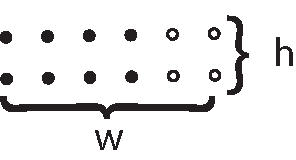
\includegraphics[width=0.24\textwidth]{img/heightwidth.pdf}
	\caption{Assumption of distribution when 4 out of 12 particles have information of destination. Circles indicates informed particles, solid dots indicates uninformed.}
	\label{fig:distr_direction}
\end{figure}
From the definition of Elongation, see \ref{sub:elongation}, we can put up a master equation for the elongation. With a distance between particles of length $\alpha$ we can define the parameters in Figure \ref{fig:distr_direction} as
\begin{align}
	h\cdot w &= N \\
	w &= (\sqrt{Np}-1)\alpha.
\end{align}
The elongation is calculated as 
\begin{equation}
	E = \frac{h}{w} = \frac{N}{(\alpha(\sqrt{Np}-1))^2}.
\end{equation}


\section{Conclusions}%
\label{sec:conc_future}
Yes

% \bibliographystyle{plain}
% \bibliography{bibliography}
% \nocite{*}

% \begin{thebibliography}{99}
% 	\bibitem{nb_thoery}\href{http://www.aaai.org/Papers/FLAIRS/2004/Flairs04-097.pdf}{Harry Zhang, The Optimality of Naive Bayes, AA, 2004}
% 	\bibitem{nb_comparison}\href{http://citeseerx.ist.psu.edu/viewdoc/download?doi=10.1.1.65.9324&rep=rep1&type=pdf}{McCallum and K. Nigam. “A Comparison of Event Models for Naive Bayes Text Classification” }
% \end{thebibliography}

\end{document}
